\documentclass[usepdftitle=false]{beamer}

\usepackage[T1]{fontenc}

\usepackage[utf8x]{inputenc}
\usepackage{default}
\usepackage{lmodern}
\usepackage{booktabs}

\usepackage{ragged2e} % Kommando\justifying ermöglicht  Blocksatz in Präsentationen

\mode<presentation>
 {\usecolortheme{seahorse,rose}
 \useinnertheme[shadow]{rounded}
%  \useoutertheme[hideothersubsections,right,width=4em,frame number]{sidebar}
%  \useoutertheme{infolines}
%\useoutertheme{split}
\useoutertheme[subsection=false,footline=authortitle]{miniframes}
\setbeamercovered{transparent}
}

%seitenzahl in linker ecke
\addtobeamertemplate{navigation symbols}{{\usebeamercolor{section
in toc}\footnotesize
\insertframenumber/\inserttotalframenumber}\hspace{48em}}{}
\usepackage{setspace} %mit spacing-Umgebung Zeilenabstand regeln



%%Sprachunterstuetzung
%Englische Silbentrennung, etc.
\usepackage[spanish]{babel}
%Mehrsprachige Literaturliste
\usepackage{babelbib}
%%Graphiken und Farbe
%Graphiken
\usepackage{graphicx} 
%von beamer.cls geladen
%Farbe
\usepackage{color,pgf}
%von beamer.cls geladen
%PDF-Seiten einbinden
\usepackage{pdfpages}
\usepackage{subscript}
\newcommand{\sub}[1]{\textsubscript{#1}}
\newcommand{\Sup}[1]{\textsuperscript{#1}}
\newcommand{\COO}{CO\textsubscript{2}}
\newcommand{\masl}{m~a.s.l.}
\newcommand{\gc}{$^{\circ}$C}
\newcommand{\tilt}{$\sim$}
\newcommand{\blue}[1]{{\color{blue!50!black}#1}}
\newcommand{\Blue}[1]{{\color{blue!50!black}\textbf{#1}}}
\newcommand{\eg}{e.\,g.}
\newcommand{\Eg}{E.\,g.}

% new environment for slides with changes margins
\newenvironment{changemargin}[2]{%
\begin{list}{}{%
\setlength{\topsep}{0pt}%
\setlength{\leftmargin}{#1}%
\setlength{\rightmargin}{#2}%
\setlength{\listparindent}{\parindent}%
\setlength{\itemindent}{\parindent}%
\setlength{\parsep}{\parskip}%
}%
\item[]}{\end{list}}





\hypersetup{
pdfauthor={Roman M. Link},
pdftitle={El sistema hidráulico de plantas},
}

%Titelseite
\title{Mediciones de hidráulica de plantas con el XylEm Plus y la bomba de Scholander}
\subtitle{\normalfont Curso de laboratorio}
\author[R. Link]{Roman Link}
\date{27 de noviembre de 2017}
\institute[University of Göttingen]{
Department of Plant Ecology and Ecosystem Research\\ Georg August University of Göttingen}
%\titlegraphic{ \vspace*{2em}
%
\includegraphics[width=0.7\textwidth]{logouni.png}}%oder was sch\"oneres

\logo{
\includegraphics[width=20em]{logounisolow.png}}

\usepackage{amsmath,amsfonts,amssymb,pgf}
 \usepackage { eulervm }

%\usepackage[round]{natbib}
%\def\newblock{} % hilft gegen absurde fehler mit natbib

\newcommand{\rar}{$\rightarrow$}
\newcommand{\lar}{$\leftarrow$}
\newcommand{\Rar}{$\Rightarrow$}
\newcommand{\Lar}{$\Leftarrow$}
\newcommand{\quelle}[1]{\baselineskip8pt{\tiny \color{gray} #1}}

\newcommand{\tw}{\textwidth}
\newcommand{\ddx}[2]{\frac{\mathrm{d}}{\mathrm{d}#2}#1 }
\newcommand{\ddxx}[2]{\frac{\mathrm{d^2}}{\mathrm{d}#2^2}#1}



\newcommand{\code}[1]{{\footnotesize \color{blue}
\texttt{#1}}\normalsize\color{black}}


% \input{cc_beamer}
\setbeamerfont{section in toc}{size=\normalsize,series=\bfseries}
\setbeamerfont{title}{series=\bfseries}
\setbeamerfont{frametitle}{size=\Large,series=\bfseries}

\begin{document}


%%%%%%%%%%%%%%%%%		Title Page			%%%%%%%%%%%%%%%%%%%%%%
\begin{frame}
\titlepage
\end{frame}

\begin{frame}
\only<1>{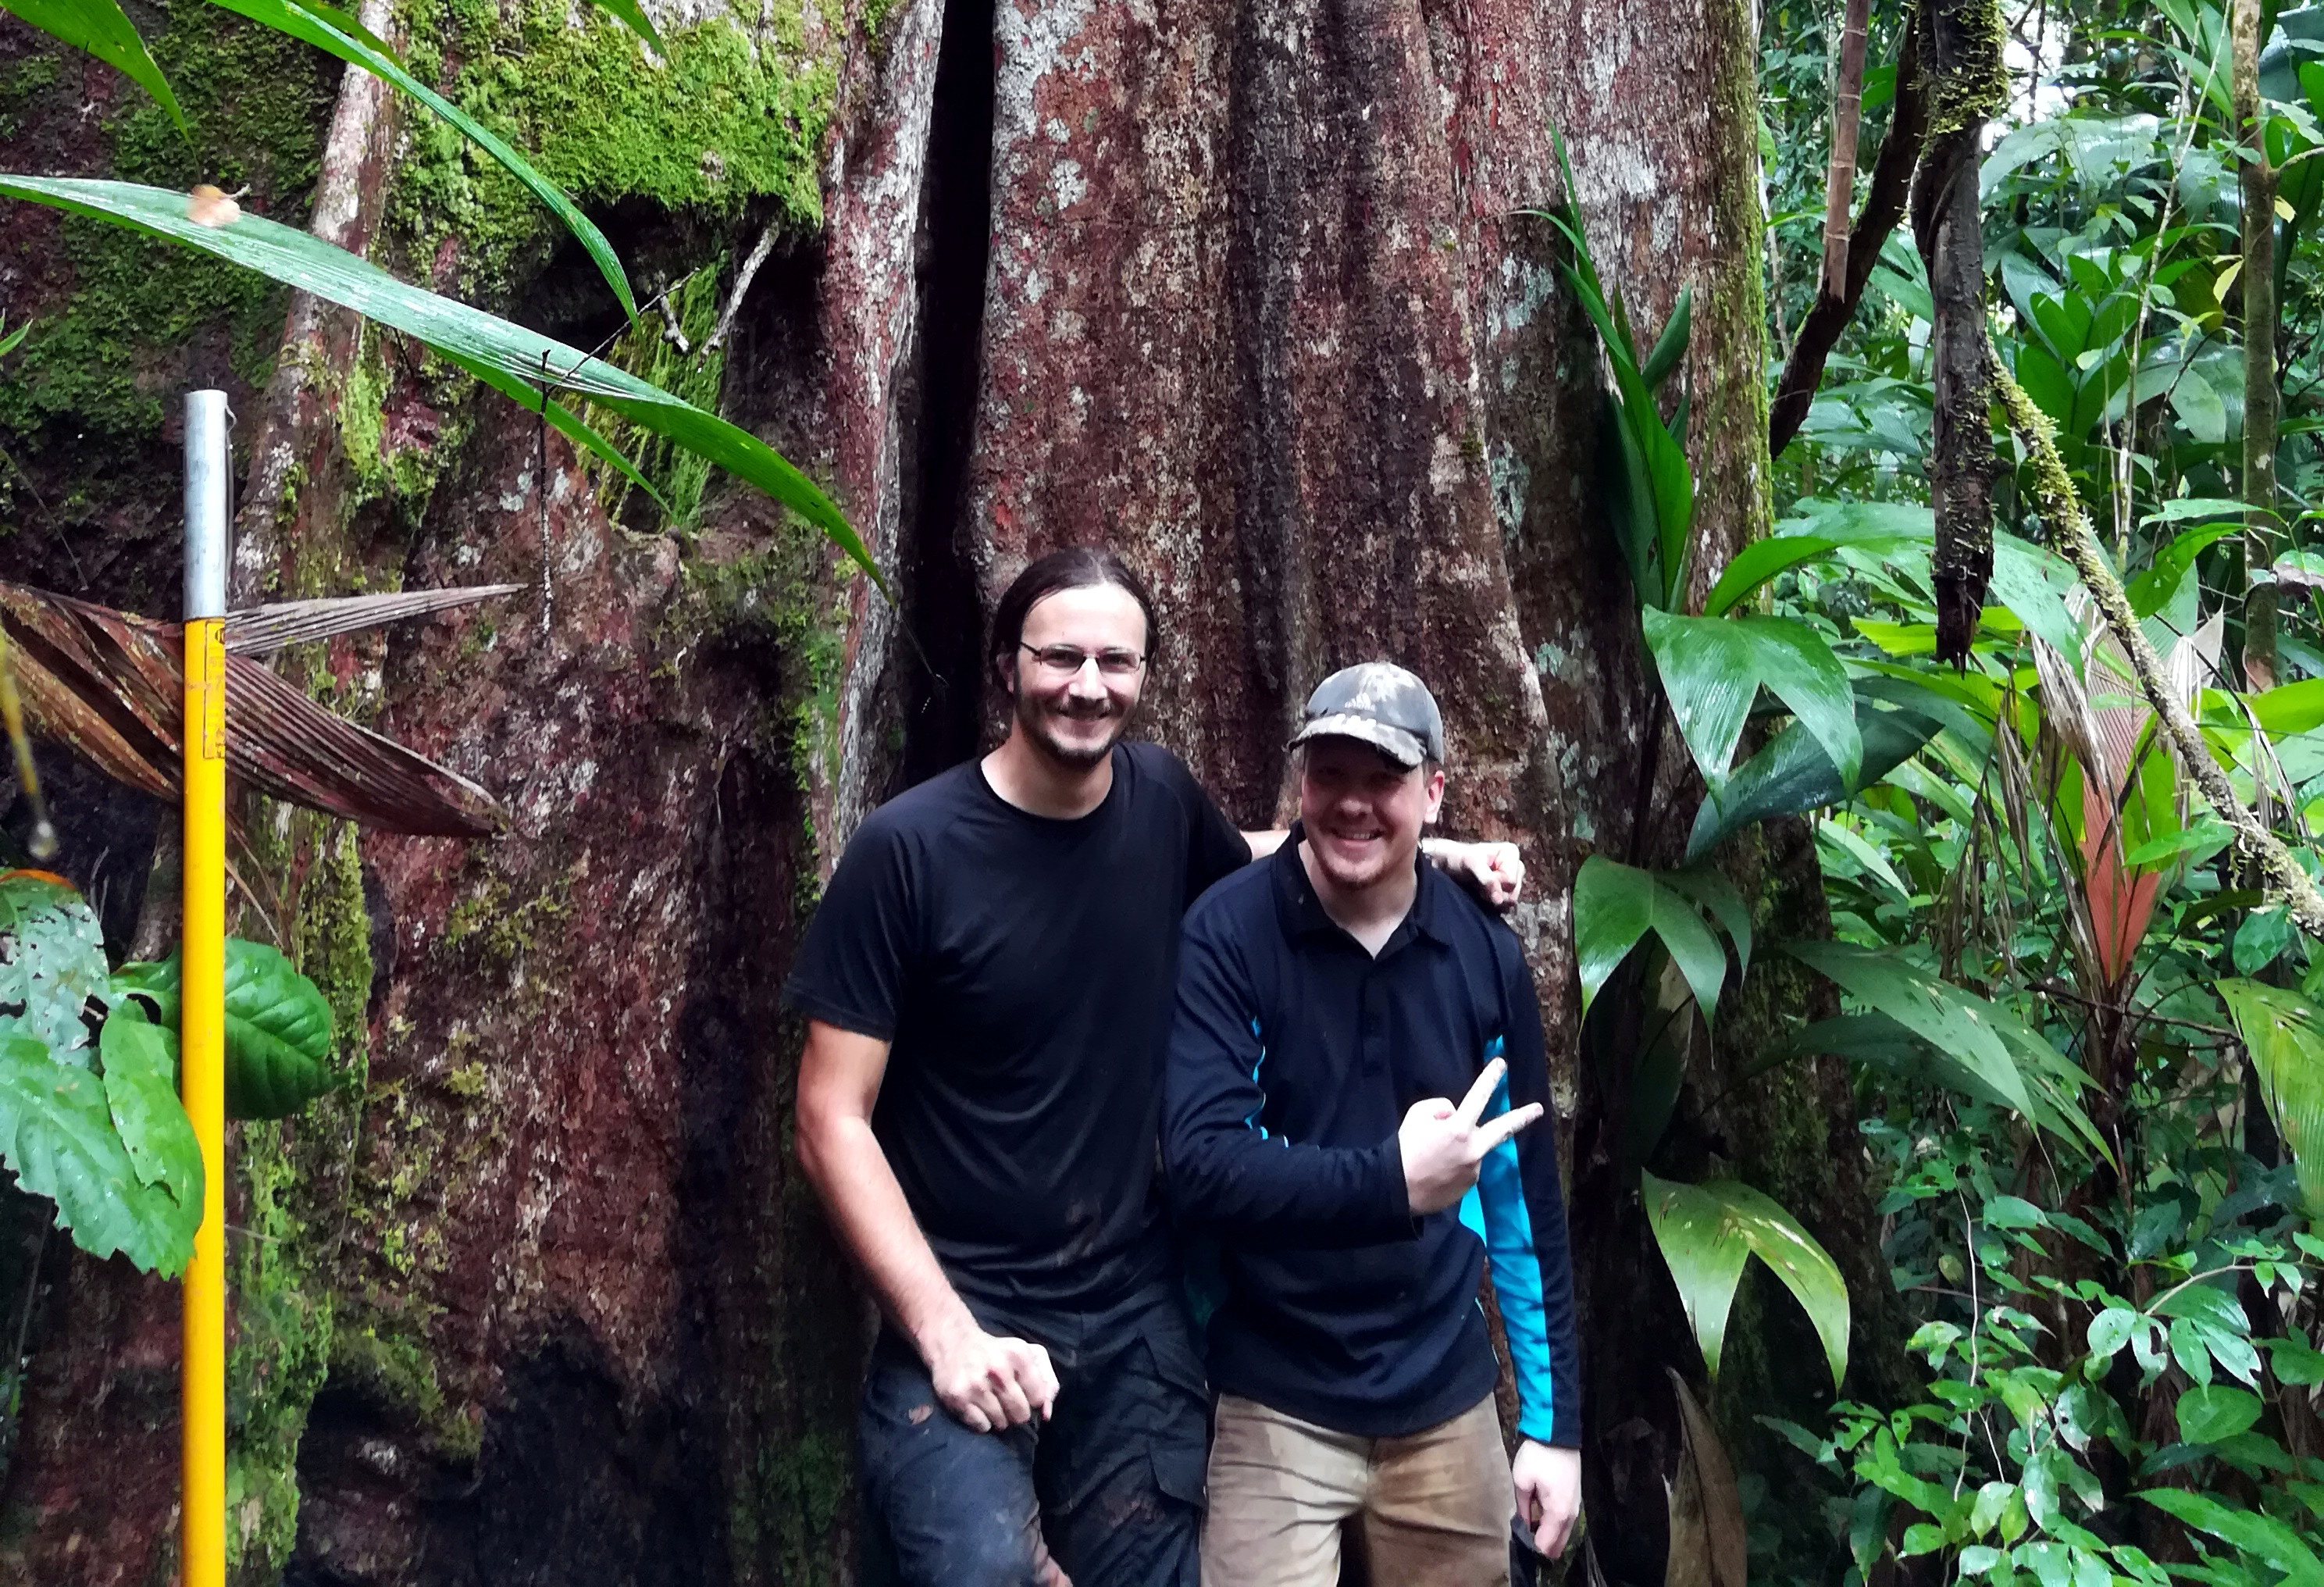
\includegraphics[width = \tw]{pictures/roman_adrian.jpg}}
\only<2>{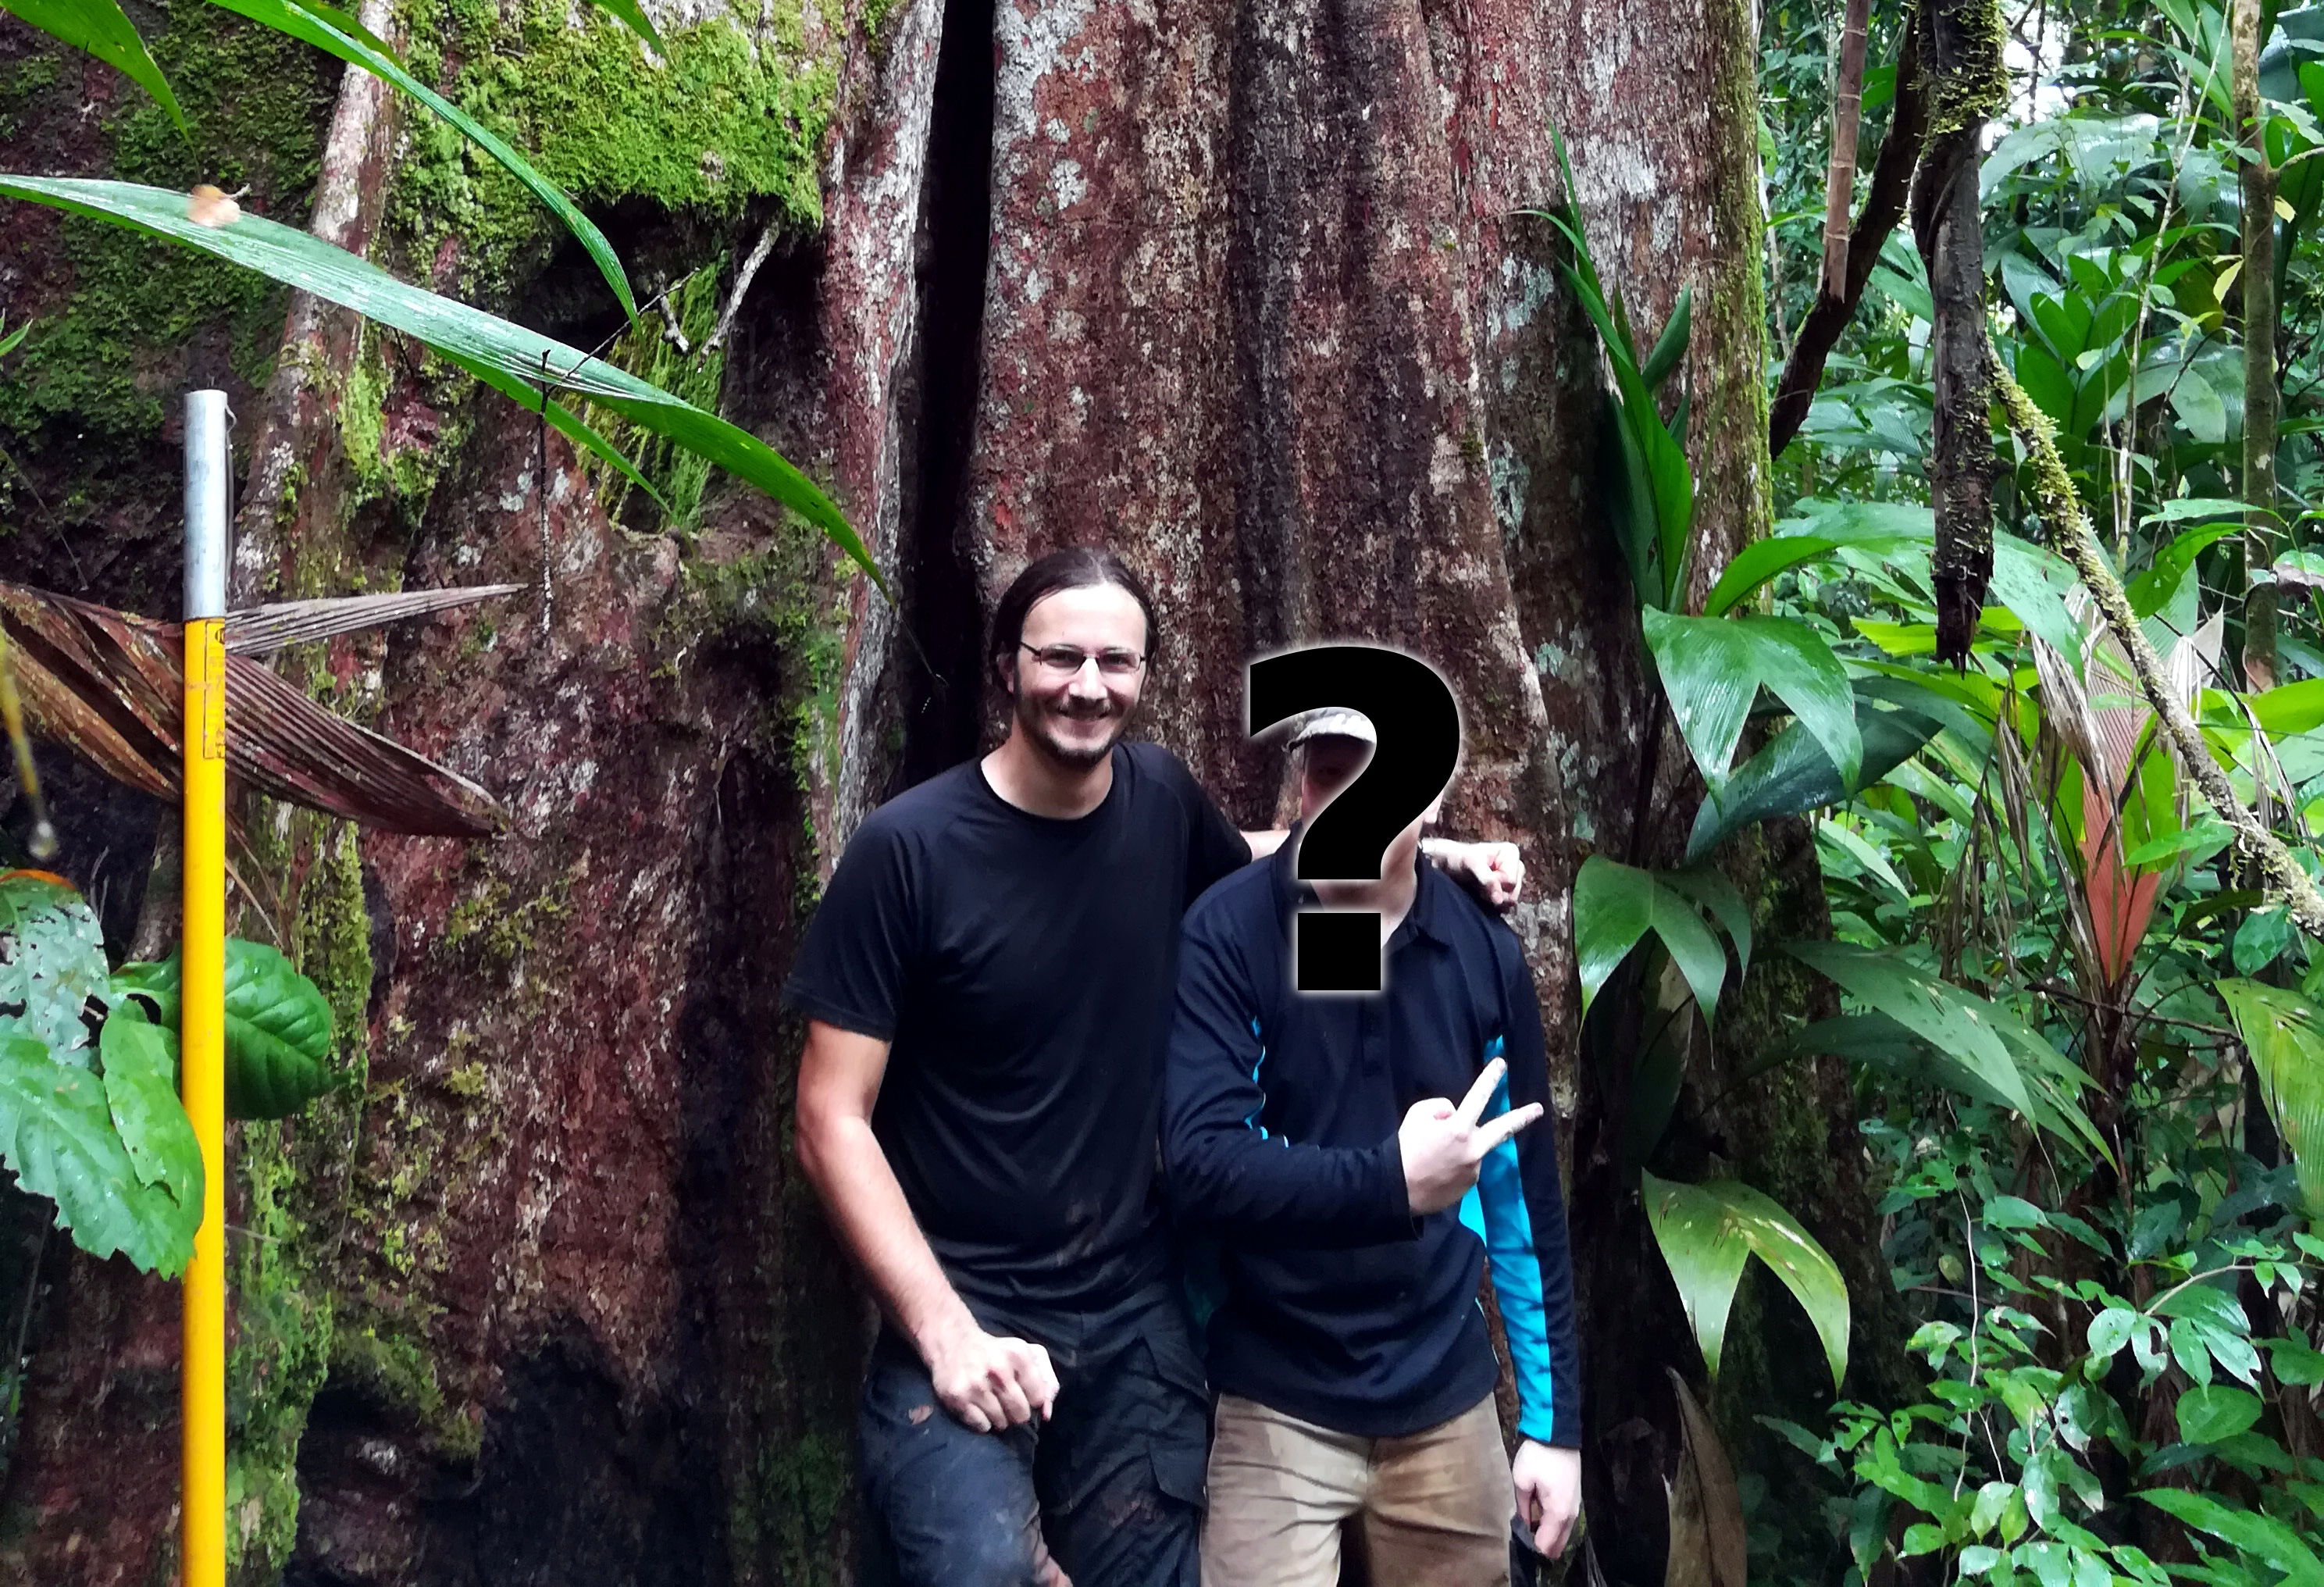
\includegraphics[width = \tw]{pictures/roman_adrian1.jpg}}
\only<3>{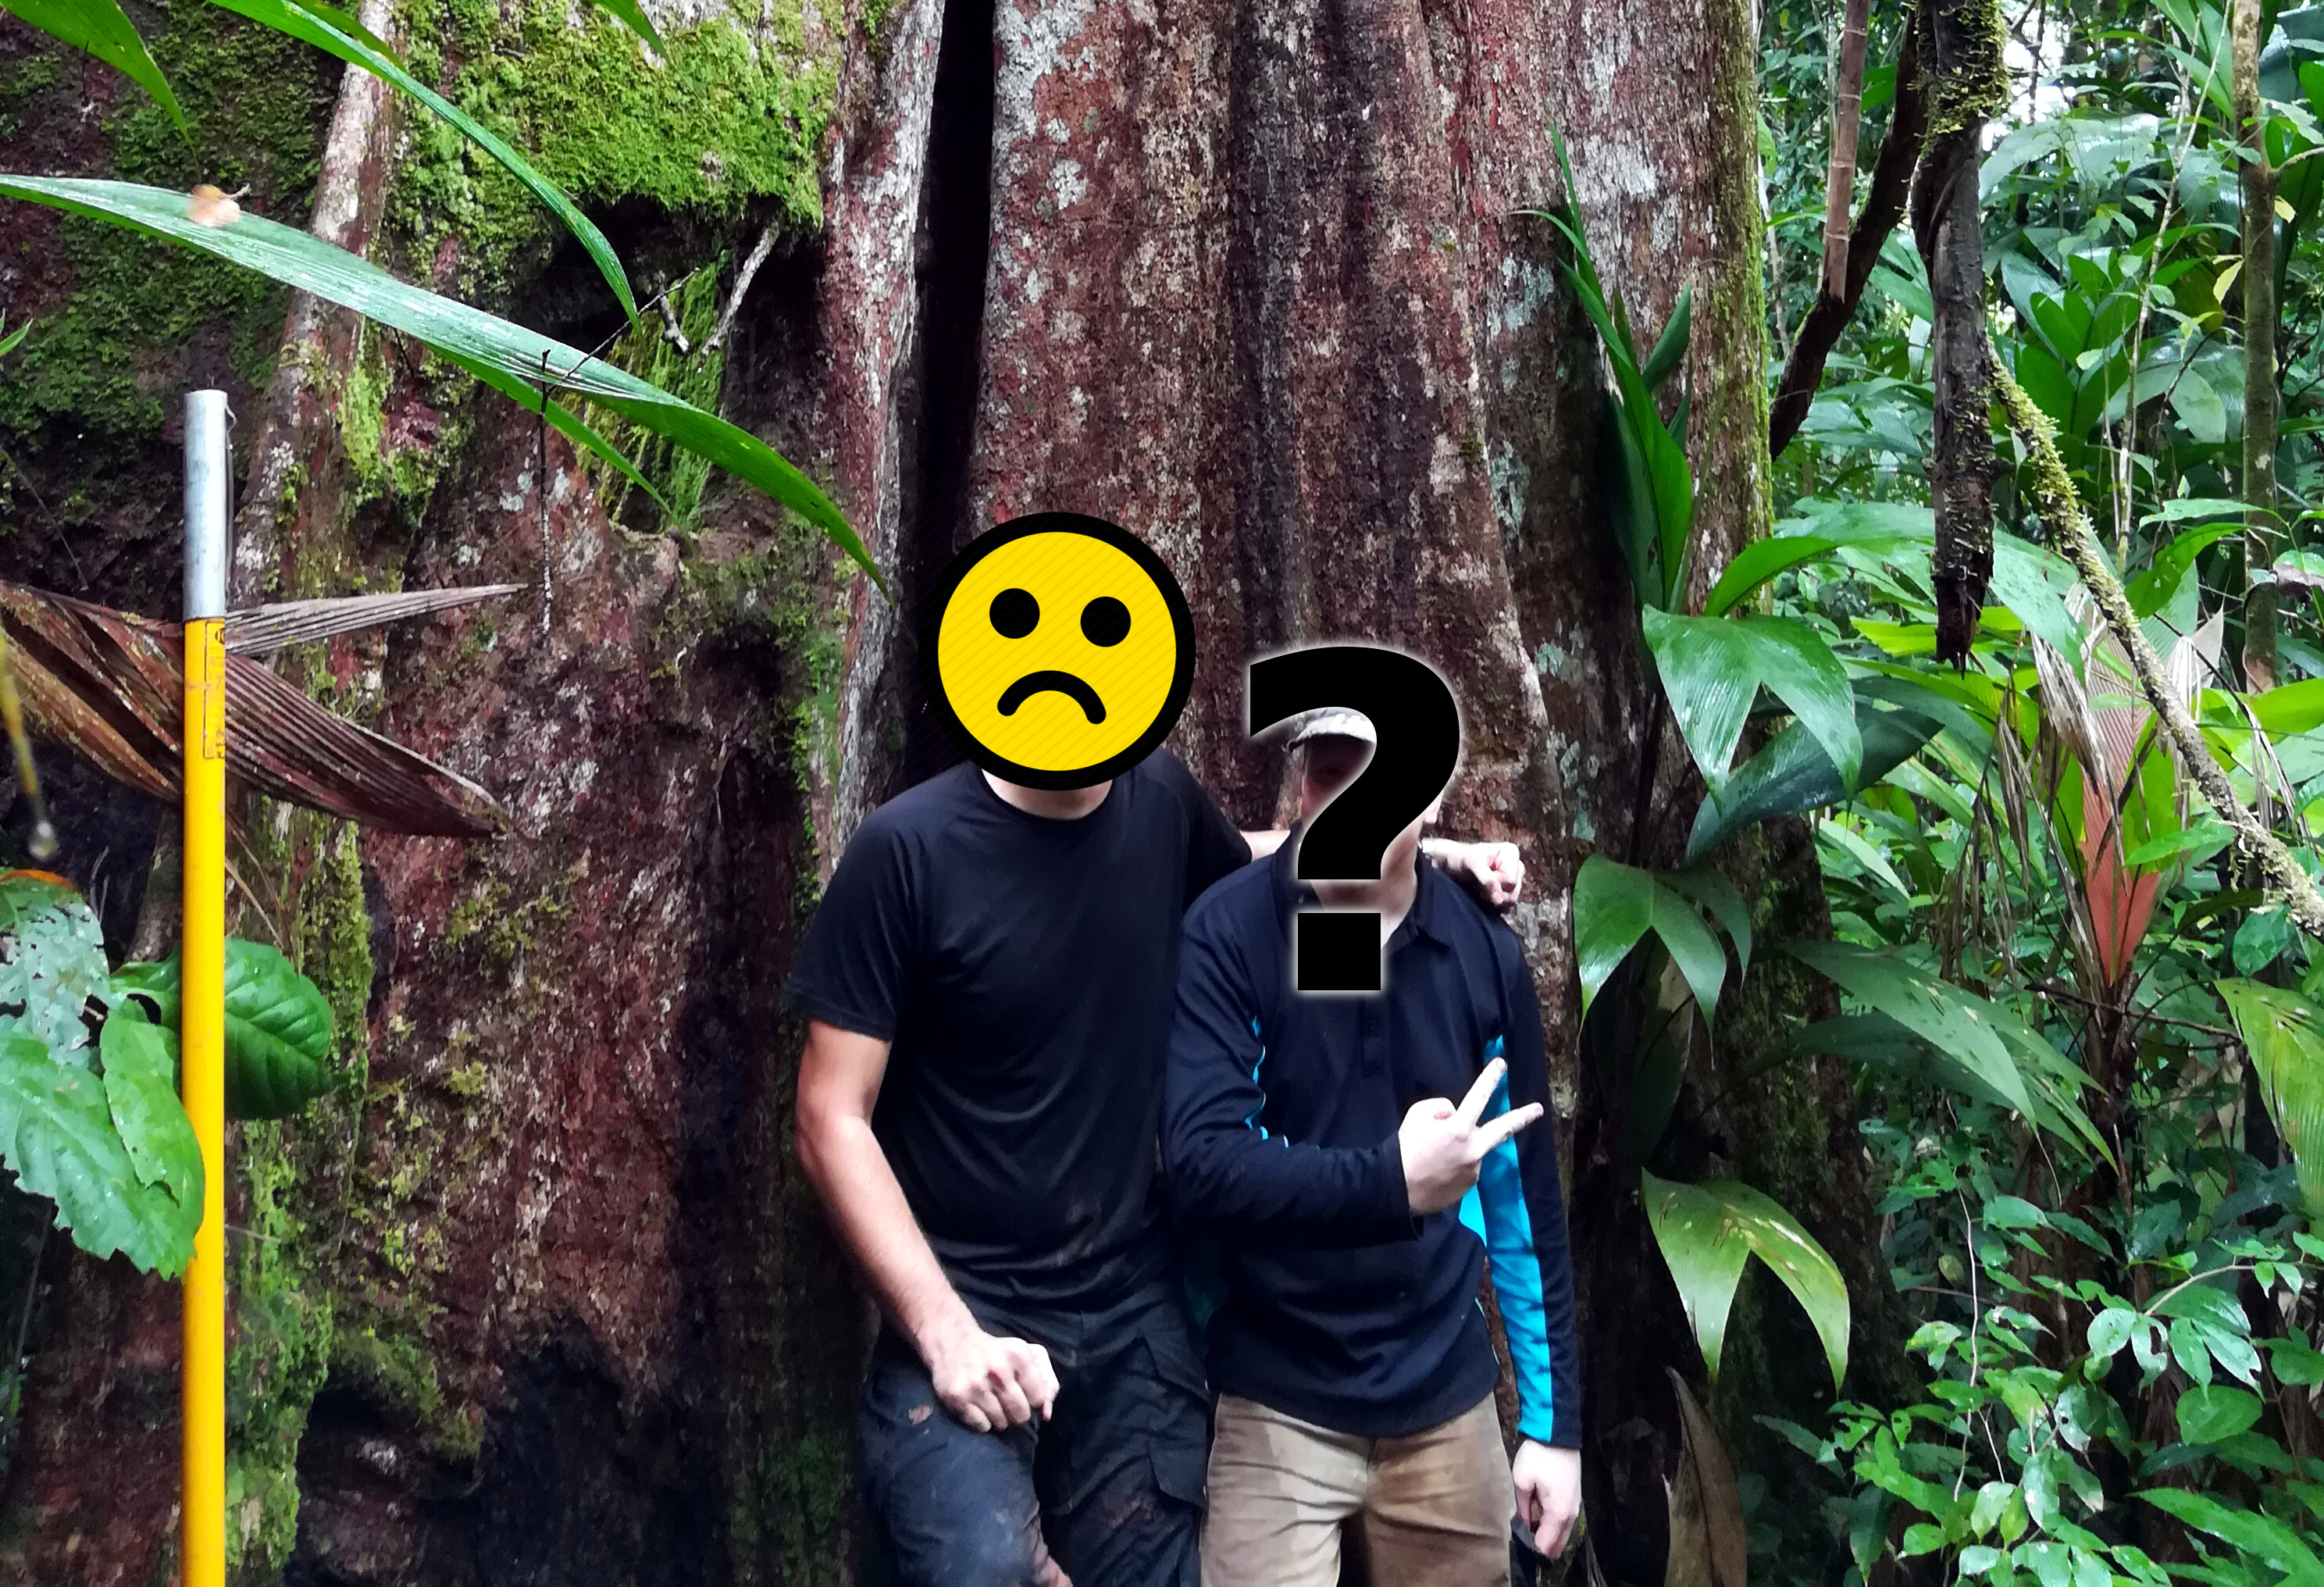
\includegraphics[width = \tw]{pictures/roman_adrian2.jpg}}
\end{frame}

\begin{frame}
	\frametitle{Estructura del curso}
	\begin{itemize}
		\item \Blue{08:30} Presentación \textit{El sistema hidráulico de plantas}
		\item \Blue{09:30} Pausa de café
		\item \Blue{10:00} Unidad \textbf{Conductividad y potencial hídrico}
		\begin{itemize}
			\item Presentación \textit{Introducción al uso del XylEm Plus y de la bomba de Scholander}
			\item Práctica de laboratorio en grupos (usando muestras de ramas de Eucalyptus sp. de las plantaciones del TEC)
			\begin{enumerate}
				\item Mediciones de conductancia/conductividad hidráulica de ramas con el XylEm Plus
				\item  Mediciones del potencial hídrico de hojas con la bomba de Scholander
			\end{enumerate}	  
	   \end{itemize}
	   \item \Blue{12:30} Pausa de almuerzo
   \end{itemize}
\end{frame}


\begin{frame}
	\frametitle{Estructura del curso}
	\begin{itemize}
		\item \Blue{13:00} Unidad \textbf{Curvas de vulnerabilidad}
		\begin{itemize}
			\item  Presentación \textit{El método de Bench Dehydration: el uso de XylEm y de la bomba de Scholander para obtener curvas de vulnerabilidad}
			\item Práctica de laboratorio en grupos (usando muestras de ramas de Eucalyptus sp. de las plantaciones del TEC)
			\begin{itemize}
				\item Preparación de muestras
				\item Mediciónes de porcientos de pérdida de conductancia (percent loss of conductivity, PLC) con el XylEm Plus
				\item Mediciones del potencial hídrico de hojas con la bomba de Scholander
			\end{itemize}
			\item Presentación \textit{Estimación de los parámetros de la curva de vulnerabilidad}
		\end{itemize}	
		\item Duración prevista del curso hasta \Blue{18:00} (dependiendo de la duración de las mediciones)	
	\end{itemize}
\end{frame}

\begin{frame}

\huge
\textbf{Materiales para el curso:}


\Blue{\url{http://bit.ly/2n8lnnJ}}

\vspace{0.5em}
\textbf{Contacto:} 

\Blue{\href{mailto:rlink@gwdg.de}{rlink@gwdg.de}}
\end{frame}
\end{document}
